%
% T�TULO DEL CAP�TULO
%
\chapter[Object detection: RANSAC]{
	Object detection: Random Sample Consensus
	\label{chapter_8}
}

RANSAC is an abbreviation for ``RANdom SAmple Consensus''. This is an iterative method to estimate parameters of a mathematical model from a set of observed points which can contain outliers. This is a non-deterministic algorithm, since we are not able to guarantee that it will produce a correct result. The probability of reaching a reasonable result will improve as the number of iterations increases. The algorithm was first published in \cite{ransac}.

The basic assumption is that the data contains \textit{inliers}\footnote{Data whose distribution can be estimated by some model.}, though it may contain noise and \textit{outliers}\footnote{Data that does not fit the model.}. Outliers can come from errors or imprecise measurements, extreme values of noise, etc. RANSAC assumes that given a set of inliers, there should exist a procedure that can estimate the unknown parameters of a model that will fit this data (see \autoref{RANSAC}).

\begin{figure}[h]
	\centering
	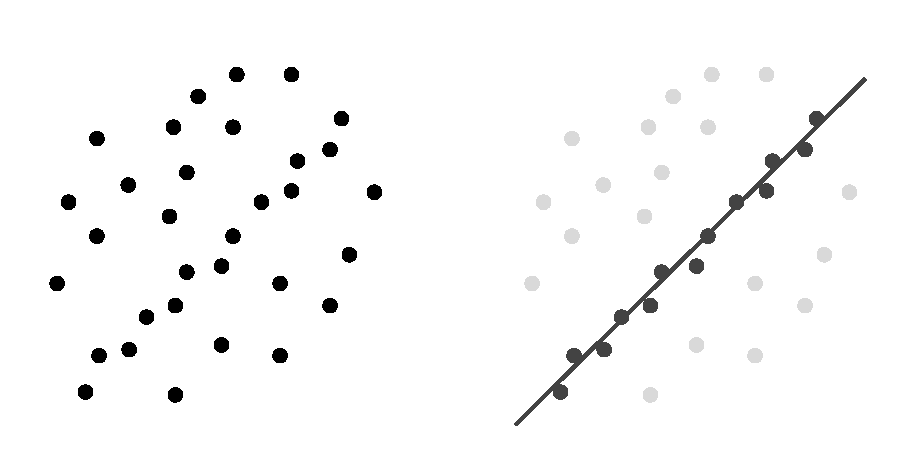
\includegraphics[scale=0.8]{figures/RANSAC.pdf}
	\caption[RANSAC example]{
		A set of points with many inliers in which a line is to be fitted (\textbf{left}).  Resulting fitted line using RANSAC, in which outliers have no influence in the result (\textbf{right}).
	}
	\label{RANSAC}
\end{figure}

\section[Original algorithm]{Original algorithm}

Unlike other estimation techniques, RANSAC generates candidate solutions using the minimum number of points required to fit the model parameters. RANSAC instead of using as much of the data as possible and then eliminate the outliers, uses the smallest set possible and then tries to enlarge this subset with coherent points. The basic algorithm can be summed up in the following steps: 

\begin{enumerate}
	\item Select randomly the minimum subset of points to determine the model parameters.
	\item Solve for the parameters of the model (i.e. with a least squares method).
	\item Test how many points from the complete dataset fit with a predefined tolerance $\epsilon$.
	\item If the fraction of inliers over the total number of points is sufficiently good, then the model is re-estimated (since it was only estimated using the initial inliers).
	\item Finally, the model is evaluated by estimating the error of the inliers relative to the model.
\end{enumerate}

This procedure is repeated a certain number of times, each time producing either a new model which is either rejected because too few points are classified as inliers or a better model together with its error measure. In the latter case, we keep the refined model if its error is lower than the last saved model.

The algorithm will stop when it reaches $N$ iterations or when the model reaches a desired error measure. $N$ can be calculated to ensure that the probability $p$ (usually 0.99) of one of the subsets of random samples will not contain an outlier. Being $u$ the probability that any selected point is an inlier and $v = 1 - u$ the probability of observing an outlier. $N$ iterations of the minimum number of points $m$ are required:

\begin{equation} 1 - p = (1 - u^m)^N \end{equation}

After solving for $N$ we will obtain the necessary number of iterations:

\begin{equation} N = \frac{log(1 - p)}{log(1 - (1 - v) ^ m)} \end{equation}

Since our objective is estimating primitives in real-time, we will let the user choose this parameter so that computational time is not too high.

An advantage of RANSAC is the robust estimation of the model parameters (it can estimate the parameters even when a significant number of outliers is present). But, a disadvantage of RANSAC is that there is no upper bound on the time that it would take to compute the correct model parameters. Another disadvantage is that it can only estimate one model at a time, if two or more instances of the model exist, RANSAC will fail to find either of them.

\section[Alternative algorithms]{Alternative algorithms}

Since 1981 RANSAC has become one of the most widely used tools in computer vision. Since then, there have been several variations of the algorithm meant to improve its robustness, speed and accuracy. Some of the improved algorithms will be briefly described in this section.

\subsection[MSAC and MLESAC]{MSAC and MLESAC}

In the original algorithm, if the threshold $\epsilon$ is too high, the robust estimate can be very poor. This happens because RANSAC finds the minimum of a cost function:

\begin{equation} C = \sum_{i} p(e_{i}^2) \end{equation}

Where $p(e^2)$ is:

\begin{equation} 
p(e^2) = \left\{\begin{matrix}
0 & e^2 < \epsilon^2\\ 
constant & e^2 \geq  \epsilon^2
\end{matrix}\right. 
\end{equation}

As we can see in the equations, inliers will score nothing and each outlier will score a constant penalty. As $\epsilon^2$ is higher, more solutions with the same value $C$ will appear, leading to worse estimations. In \cite{robustparam} it is shown that this can be avoided changing $C$ for:

\begin{equation} C_{2} = \sum_{i} p_{2}(e_{i}^2) \end{equation}

Where $p_{2}(e^2)$ is:

\begin{equation} 
p_{2}(e^2) = \left\{\begin{matrix}
e^2 & e^2 < \epsilon^2\\ 
\epsilon^2 & e^2 \geq  \epsilon^2
\end{matrix}\right. 
\end{equation}

This is known as a re-descending M-estimator. Outliers are still given a constant penalty, but now inliers are scored depending on how well they fit the data. The implementation of this method is called MSAC\footnote{M-Estimator Sample Consensus}.

The definition of a maximum likelihood error, will allow to further improve the results of this new technique. This improved technique is called MLESAC\footnote{Maximum Likelihood Sample Consensus} \cite{MLESAC}. The improved algorithm steps are:

\begin{enumerate}
	\item Get the minimum number of samples that will satisfy the model criteria.
	\item Search for inliers.
	\item Calculate distances to the model.
	\item Use Expectation-Maximization to find out the right value for the penalty.
	\item If the fraction of inliers over the total number of points is sufficiently good, then the model is re-estimated (since it was only estimated using the initial inliers).
	\item Finally, the model is evaluated by estimating the error of the inliers relative to the model.
\end{enumerate}
 
It can be seen that MSAC and MLESAC outperform the other two estimators, providing a $5 - 10\%$ improvement according to \cite{MLESAC}.

\subsection[PROSAC]{PROSAC}

PROSAC\footnote{Progressive Sample Consensus} is a new robust method, that exploits the linear ordering in a set of candidates using a similarity function for this purpose \cite{PROSAC}. On one hand, RANSAC normally treats all correspondences as equals and drawing uniform random samples from the dataset. On the other hand, PROSAC samples are drawn from progressively bigger sets of the best ranked candidates.

Usually, RANSAC will generate $N$ candidates. The set of $\varepsilon$ candidates, will contain a now unknown number of inliers $I$. The RANSAC loop is terminated when the probability of finding a better solution falls under a predetermined threshold. The average number of samples drawn is proportional to $(N/I)^m$. This method will be less expensive computationally than the original RANSAC, by using the linear order in $\varepsilon$. The set of candidates is obtained evaluating a similarity function $q(\cdot)$. After this step, the candidates are ordered according to the quality function. The algorithm will evaluate $N$ candidates like RANSAC, but it will do it in a different order, the samples that are of higher quality (less contaminated) will be examined first. The function chosen $q(\cdot)$ can be the Euclidean distance or any other similarity metric. 

The algorithm steps are in this case:

\begin{enumerate}
	\item Choose the hypothesis generation set.
	\item Generate hypothesis using random sampling (drawn from the subset of high quality data).
	\item Search for inliers using the estimated model.
	\item Model verification.
	\item If the probability of finding a better solution falls below a threshold terminate.
\end{enumerate}

According to \cite{PROSAC}, PROSAC is more than a hundred times faster than RANSAC in non-trivial cases.

\subsection[RRANSAC]{RRANSAC}

Typically, RANSAC will spend a lot of computational resources evaluating a large number of erroneous candidate models. These erroneous models will only fit a small subset of the complete dataset. This fact is exploited in \cite{RRANSAC} to create RRANSAC and significantly increase the speed of the original algorithm. 

The main concept in this technique, is that the efficiency of the algorithm will be improved substantially when the hypothesis evaluation step is randomized. What this means, is that because most of the hypothesis are influenced by outliers, testing a small number of points $d$ from the total $N$ ($d \ll N$) will suffice to discard the bad solution.

This idea is implemented in a two-step evaluation procedure. First, a statistical test is performed on $d$ randomly selected data points. Second, the evaluation of all the points in the dataset is only performed if the pre-test is passed. The preverification test is called the $T_{d,d}$ test, and is passed only when $d$ data points out of $d$ randomly selected are consistent with the hypothesis. 

The only remaining task is knowing the optimal value of $d$. The following equation will yield that value:

\begin{equation} d^* \approx \frac{\ln(\frac{\ln \varepsilon (t_{M}+1)}{N (\ln \delta - \ln \varepsilon)})}{\ln \delta} \end{equation}

Being $\varepsilon$ the fraction of inliers in the dataset, $\delta$ the probability that a data point is consistent with a ``random'' model and $t_{M}$ is the time needed to compute the parameters of the model from the selected samples. 

The algorithm steps in this instance are:

\begin{enumerate}
	\item Choose the hypothesis generation set.
	\item Generate hypothesis using random sampling.
	\item Perform the pre-test on $d$ points.
	\item Model verification only if test is passed.
	\item If the probability of finding a better solution falls below a threshold terminate.
\end{enumerate}

It is interesting to mention that the speed boost of this algorithm can be combined with the more robust estimation of MSAC, resulting in a variation called RMSAC. This method combines the best properties of these two techniques, yielding fast and robust estimations. 
 
\section[Point-primitive distance calculation]{Point-primitive distance calculation}

Once the parameters of a model are estimated, a evaluation of the solution has to be performed. In order to do this, the outliers and inliers will be calculated. To know if a point is an outlier or an inlier, the distance from the point to the surface of the primitive will have to be computed. In the following subsections the math needed to measure the distance from planes, cylinders and spheres to a point will be explained.

\subsection[Point-plane distance]{Point-plane distance}  

The chosen convention to express the parameters of the plane is the \textit{Hessian normal form}. These parameters will specify an infinite plane, that will have to have its length limited later on, in order for it to be used in the CAD exportation. 

\begin{figure}[h]
	\centering
	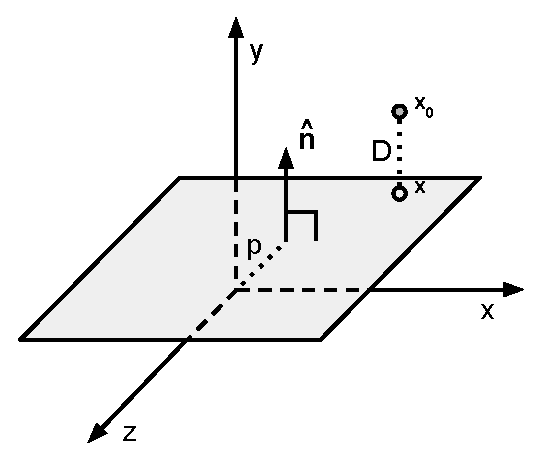
\includegraphics[scale=0.9]{figures/hessian.pdf}
	\caption[Hessian normal form]{
		Visual explanation of the parameters involved in the distance calculation from a point to a plane in Hessian normal form.
	}
	\label{hessian}
\end{figure}

This form can obtained calculating several parameters using the general parametric equation of a plane:

\begin{equation} ax + by + cz + d = 0 \end{equation}

Thanks to this equation we can define the \textit{unit normal vector} $\mathbf{\hat{n}}$:

\begin{equation} \mathbf{\hat{n}} = (n_{x},n_{y},n_{z}) \end{equation}

Being $n_{x}$, $n_{y}$ and $n_{z}$:

\begin{equation} 
\begin{matrix}
n_{x} = \frac{a}{\sqrt{a^2 + b^2 + c^2}}
\\ 
n_{y} = \frac{b}{\sqrt{a^2 + b^2 + c^2}}
\\ 
n_{z} = \frac{c}{\sqrt{a^2 + b^2 + c^2}}
\end{matrix}
\end{equation}

And the constant $p$:

\begin{equation} p = \frac{d}{\sqrt{a^2 + b^2 + c^2}} \end{equation}

Then the Hessian normal form of a plane is:

\begin{equation}\label{eq:hessian} \mathbf{\hat{n}} \cdot \mathbf{x} = -p \end{equation}

Once we have the Hessian normal form parameters (see \autoref{hessian}) and a point $\mathbf{x_{0}}$, the point-plane distance $D$ is given by the following equation:

\begin{equation} D = \mathbf{\hat{n}} \cdot \mathbf{x_{0}} + p \end{equation}

\subsection[Point-cylinder distance]{Point-cylinder distance} 

In the case of the cylinder, the parameters chosen to represent it can be seen in \autoref{cyl_dist}. These parameters will specify an infinite cylinder, that will have to be bound later in order for it to be useful.

\begin{figure}[h]
	\centering
	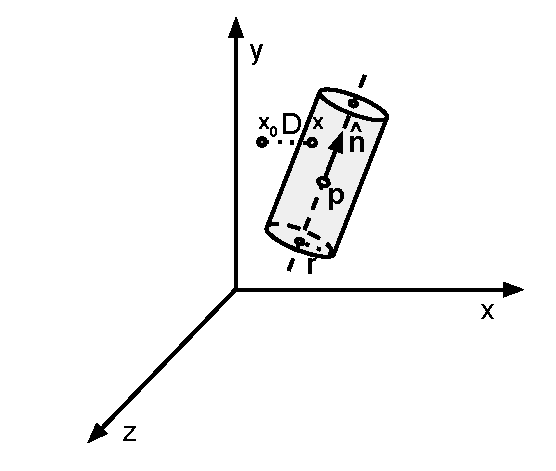
\includegraphics[scale=1]{figures/cylinder_dist.pdf}
	\caption[Cylinder parameters]{
		Visual representation of the parameters involved in the point-cylinder distance calculation.
	}
	\label{cyl_dist}
\end{figure}    

The parameter $\mathbf{\hat{n}} = (n_{x},n_{y},n_{z})$ represents the \textit{unit normal vector} of its axis, $\mathbf{p} = (p_{x},p_{y},p_{z})$ a point on its axis and $\mathbf{r}$ its radius. Furthermore, if we define two more unit vectors $\mathbf{\hat{u}}$ and $\mathbf{\hat{v}}$ as a right-handed orthonormal set $\left \{ \mathbf{\hat{u}}, \mathbf{\hat{v}}, \mathbf{\hat{n}} \right \}$, then any point in the cylinder $\mathbf{x}$ can be written as:

\begin{equation} \mathbf{x} = \mathbf{p} + \mathbf{\hat{u}}x + \mathbf{\hat{v}}y + \mathbf{\hat{n}}z \end{equation}

Once we have every parameter and a point $\mathbf{x_{0}}$, we can calculate the distance $D$ with the following equation:

\begin{equation} D = \lVert \mathbf{\hat{n}} \times (\mathbf{x_{0}} - \mathbf{p}) \rVert \end{equation}

\subsection[Point-sphere distance]{Point-sphere distance} 

For spheres, the parameters chosen to represent the estimated primitive can be seen in \autoref{sph_dist}. 

\begin{figure}[h]
	\centering
	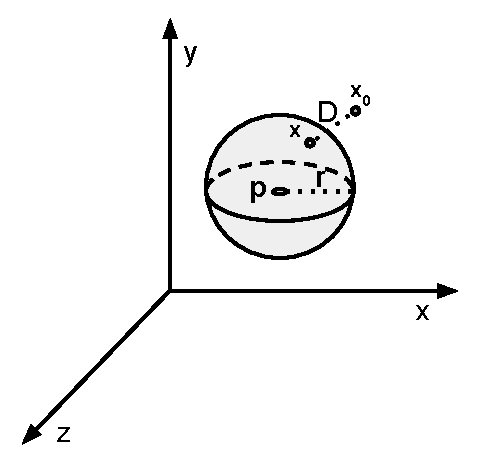
\includegraphics[scale=1]{figures/sphere_dist.pdf}
	\caption[Sphere parameters]{
		Visual explanation of the parameters involved in the point-sphere distance calculation.
	}
	\label{sph_dist}
\end{figure}

The parameter $\mathbf{p} = (p_{x},p_{y},p_{z})$ represents the center of the sphere and $\mathbf{r}$ the radius. The Cartesian equation of a sphere centered in $\mathbf{p}$ is:

\begin{equation} (x - p_{x})^2 + (y - p_{y})^2 + (z - p_{z})^2 = \mathbf{r}^2 \end{equation}

When we have every parameter and a point $\mathbf{x_{0}}$, we can calculate the distance $D$ with the next equation:

\begin{equation} D = \lVert \mathbf{x_{0}} - \mathbf{p} \rVert - r\end{equation}

\section[Primitive bounding]{Primitive bounding}

Due to the fact that parametric cylinders and planes are infinite, in order to export them to CAD software we need to bound them. Therefore, we will use the bounding box of the complete dataset to establish these boundaries.

\subsection[Plane bounding]{Plane bounding} 

To bound a plane, we will have to calculate the intersection between the \textit{AABB}\footnote{Axis Aligned Bounding Box} of the scene and a plane. This intersection will yield a three to six vertex polyline\autoref{plane_bound}. 

\begin{figure}[h]
	\centering
	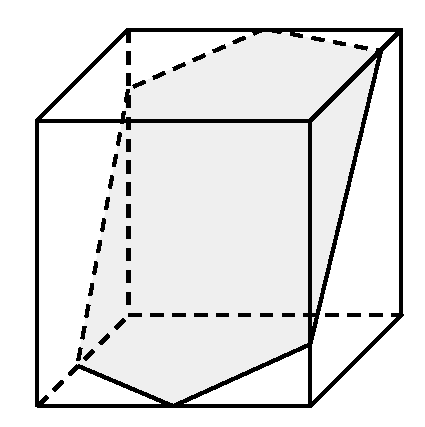
\includegraphics[scale=1]{figures/plane_bound.pdf}
	\caption[AABB-plane intersection]{
		Visual representation of a AABB-plane intersection.
	}
	\label{plane_bound}
\end{figure}

In order to obtain the polyline vertices, we will intersect every edge with the plane. This means that a common ray-plane intersection test has to be performed for each edge (see \autoref{ray_plane}). The point of intersection in the plane can be written as in \autoref{eq:hessian} and in the ray can be written as:  

\begin{equation} \mathbf{x} = \mathbf{x_{0}} + t \mathbf{\hat{v}} \end{equation}

\begin{figure}[h]
	\centering
	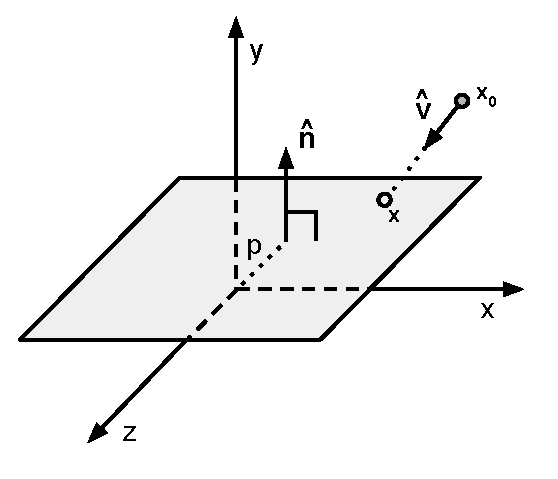
\includegraphics[scale=1]{figures/ray_plane_int.pdf}
	\caption[Ray-plane intersection]{
		Visual representation of a ray-plane intersection.
	}
	\label{ray_plane}
\end{figure}

Being $\mathbf{x_{0}}$ the origin of the ray, $\mathbf{\hat{v}}$ the direction and $t$:

\begin{equation} t = \frac{-(\mathbf{x_{0}} \cdot \mathbf{\hat{n}} + p)}{\mathbf{\hat{v}} \cdot \mathbf{\hat{n}}} \end{equation}

Once all the intersection points have been obtained, they are tested to check if they fall inside the AABB. After this we will have the vertices of the bounded plane ready to be exported.

\subsection[Cylinder bounding]{Cylinder bounding} 







  